% This is "sig-alternate.tex" V2.1 April 2013
% This file should be compiled with V2.5 of "sig-alternate.cls" May 2012
%
% This example file demonstrates the use of the 'sig-alternate.cls'
% V2.5 LaTeX2e document class file. It is for those submitting
% articles to ACM Conference Proceedings WHO DO NOT WISH TO
% STRICTLY ADHERE TO THE SIGS (PUBS-BOARD-ENDORSED) STYLE.
% The 'sig-alternate.cls' file will produce a similar-looking,
% albeit, 'tighter' paper resulting in, invariably, fewer pages.
%
% ----------------------------------------------------------------------------------------------------------------
% This .tex file (and associated .cls V2.5) produces:
%       1) The Permission Statement
%       2) The Conference (location) Info information
%       3) The Copyright Line with ACM data
%       4) NO page numbers
%
% as against the acm_proc_article-sp.cls file which
% DOES NOT produce 1) thru' 3) above.
%
% Using 'sig-alternate.cls' you have control, however, from within
% the source .tex file, over both the CopyrightYear
% (defaulted to 200X) and the ACM Copyright Data
% (defaulted to X-XXXXX-XX-X/XX/XX).
% e.g.
% \CopyrightYear{2007} will cause 2007 to appear in the copyright line.
% \crdata{0-12345-67-8/90/12} will cause 0-12345-67-8/90/12 to appear in the copyright line.
%
% ---------------------------------------------------------------------------------------------------------------
% This .tex source is an example which *does* use
% the .bib file (from which the .bbl file % is produced).
% REMEMBER HOWEVER: After having produced the .bbl file,
% and prior to final submission, you *NEED* to 'insert'
% your .bbl file into your source .tex file so as to provide
% ONE 'self-contained' source file.
%
% ================= IF YOU HAVE QUESTIONS =======================
% Questions regarding the SIGS styles, SIGS policies and
% procedures, Conferences etc. should be sent to
% Adrienne Griscti (griscti@acm.org)
%
% Technical questions _only_ to
% Gerald Murray (murray@hq.acm.org)
% ===============================================================
%
% For tracking purposes - this is V2.0 - May 2012

\documentclass{sig-alternate-05-2015}
\usepackage{float}
\floatplacement{figure}{H} % force figures to be placed always at defined position!

\begin{document}

% Copyright
%\setcopyright{acmcopyright}
%\setcopyright{acmlicensed}
%\setcopyright{rightsretained}
%\setcopyright{usgov}
%\setcopyright{usgovmixed}
%\setcopyright{cagov}
%\setcopyright{cagovmixed}


% DOI
%\doi{10.475/123_4}

% ISBN
%\isbn{123-4567-24-567/08/06}

%Conference
%\conferenceinfo{PLDI '13}{June 16--19, 2013, Seattle, WA, USA}

%\acmPrice{\$15.00}

%
% --- Author Metadata here ---
%\conferenceinfo{WOODSTOCK}{'97 El Paso, Texas USA}
%\CopyrightYear{2007} % Allows default copyright year (20XX) to be over-ridden - IF NEED BE.
%\crdata{0-12345-67-8/90/01}  % Allows default copyright data (0-89791-88-6/97/05) to be over-ridden - IF NEED BE.
% --- End of Author Metadata ---

\title{Reads Optimized LSM-tree In C}
\subtitle{Development Project - CS 265}
%
% You need the command \numberofauthors to handle the 'placement
% and alignment' of the authors beneath the title.
%
% For aesthetic reasons, we recommend 'three authors at a time'
% i.e. three 'name/affiliation blocks' be placed beneath the title.
%
% NOTE: You are NOT restricted in how many 'rows' of
% "name/affiliations" may appear. We just ask that you restrict
% the number of 'columns' to three.
%
% Because of the available 'opening page real-estate'
% we ask you to refrain from putting more than six authors
% (two rows with three columns) beneath the article title.
% More than six makes the first-page appear very cluttered indeed.
%
% Use the \alignauthor commands to handle the names
% and affiliations for an 'aesthetic maximum' of six authors.
% Add names, affiliations, addresses for
% the seventh etc. author(s) as the argument for the
% \additionalauthors command.
% These 'additional authors' will be output/set for you
% without further effort on your part as the last section in
% the body of your article BEFORE References or any Appendices.

\numberofauthors{1} %  in this sample file, there are a *total*
% of EIGHT authors. SIX appear on the 'first-page' (for formatting
% reasons) and the remaining two appear in the \additionalauthors section.
%
\author{
% You can go ahead and credit any number of authors here,
% e.g. one 'row of three' or two rows (consisting of one row of three
% and a second row of one, two or three).
%
% The command \alignauthor (no curly braces needed) should
% precede each author name, affiliation/snail-mail address and
% e-mail address. Additionally, tag each line of
% affiliation/address with \affaddr, and tag the
% e-mail address with \email.
%
% 1st. author
\alignauthor
Nicolas Drizard\\
       \affaddr{Harvard University}\\
       \email{nicolasdrizard@g.harvard.edu}
}
% There's nothing stopping you putting the seventh, eighth, etc.
% author on the opening page (as the 'third row') but we ask,
% for aesthetic reasons that you place these 'additional authors'
% in the \additional authors block, viz.

% Just remember to make sure that the TOTAL number of authors
% is the number that will appear on the first page PLUS the
% number that will appear in the \additionalauthors section.

\maketitle
\begin{abstract}
This project aims to build a data structure providing low-cost indexing for a file experiencing a high rate of record inserts/deletes over an extended period: a Log-Structured Merge-tree (LSM-tree) presented in \cite{lsm}. Efficient memory based data structure are not possible with a large number of records, especially being able to access any element is a requirement of the system. The LSM-Tree faces the challenge as it operates on batch for the inserts/updates, cascading the changes from its first compononent $C_0$ (memory based) to one or more larger components (disk-based). In this implementation, each component uses a sorted array (except for the first component) as data structure and the data operation READ, INSERT, UPDATE and DELETE are handled. The focus was on both having fast operations and a persistent implementation. The update rate is about 0.25M per second and the read rate about 22,5 K per second on flash storage.

\end{abstract}


%
%  Use this command to print the description
%
%\printccsdesc

% We no longer use \terms command
%\terms{Theory}

\keywords{LSM tree, Bloom Filter}

\section{Introduction}

Traditionnaly, transactional log records face a high rate of inserts and updates but less read operations. The number of elements keeps increasing and each of them needs to be stored persistently. As a result, solutions using memory-resident data structures are not feasible. For instance, a web merchant history may be based on this data structure, logging the purchases of the users. More and more events will be added to the structure but only a few will be read or delete but nonetheless all the past need to be accessible in case.

The multi-component LSM-trees implemented in this paper provide promising results for the targeted behavior. The key-value storage is handled with one continuous sorted array at each component level. We use two components on memory: $C_0$ and a buffer. We set a fixed number of components on disk and their size is a user-defined parameter. The operations insert/update/delete apply the same routine over the structure. Duplicated keys are removed when merging a component into another, otherwise the key in the lowest component is always considered in the reads. Another merging strategy is considered with a fixed number of independent arrays per component, merged all at once when moving to the next component. This should be more write-optimized as we merge less often but the reads are more expansive as more independent sorted arrays need to be scanned.

This paper covers in details in the first part the design of the implementation, presents the experimental results in the second part and exposes next steps in the conclusion.

\section{Design}

This part presents the design chosen for this implementation. The LSM tree structure still gives a lot of freedom depending on the tradeoffs between writes and reads expected by the user.

\subsection{Data Structure}

One of the first design questions concerns the data structure used in the two types of components ($C_0$ the entry component in memory, and $C_i$ on disk). An intuitive choice for $C_0$ is an array as we there is no need to keep it sorted, we just append each entry to it. The deeper components need an index-based structure. My approach is to use a sorted array at each level. The data structure is a key-values store. To minimize the number of scan during the merges and the reads I store in two different arrays the keys and the values.

Once the data structure of each component is defined, we need to define also metadata of our LSM Tree. These metadata will contain the following information:
\begin{itemize}
	\item value size (int value\_size);
	\item number of element (long Ne);
	\item number of components (long Nc);
	\item array of the components size(int Cs\_size[]);
	\item array of the components number of elements (int Cs\_Ne[])
	\item the bloom filter (its size, count of activated bits and table)
\end{itemize}
			
\subsection{Operations}
The LSM Tree need to support INSERT, READ, UPDATE and DELETE. We will treat similarly the INSERT, UPDATE and DELETE operations as an APPEND operation.

\paragraph{APPEND}
These operations aim to add/retrieve to the Tree a tuple (key, value). The key may be already stored but the overall approach is the same. The delete operation append the key associated to a tombstone value. For insert/delete, we first do a linear scan of $C_0$ and if the key is found there we proceed to an in-place operation. Otherwise, we append the key to the unsorted $C_0$ component. We will delete it from its cell in the corresponding component. If $C_0$ reaches its threshold we flush it into the buffer.

The merging strategy when flushing a component to a lower one is another key choice. The core solution I implemented keeps one single array of keys for each component, with a size being a multiple of the array size of the component above it. This decision will benefit to the reads as we keep a single indexed structure for each component. The write may be more expensive as we have to do a binary merge of two sorted arrays each time we flush. The step-by-step process is described in the figure \ref{fig:merge}.

\begin{figure}[H]%
\begin{center}
    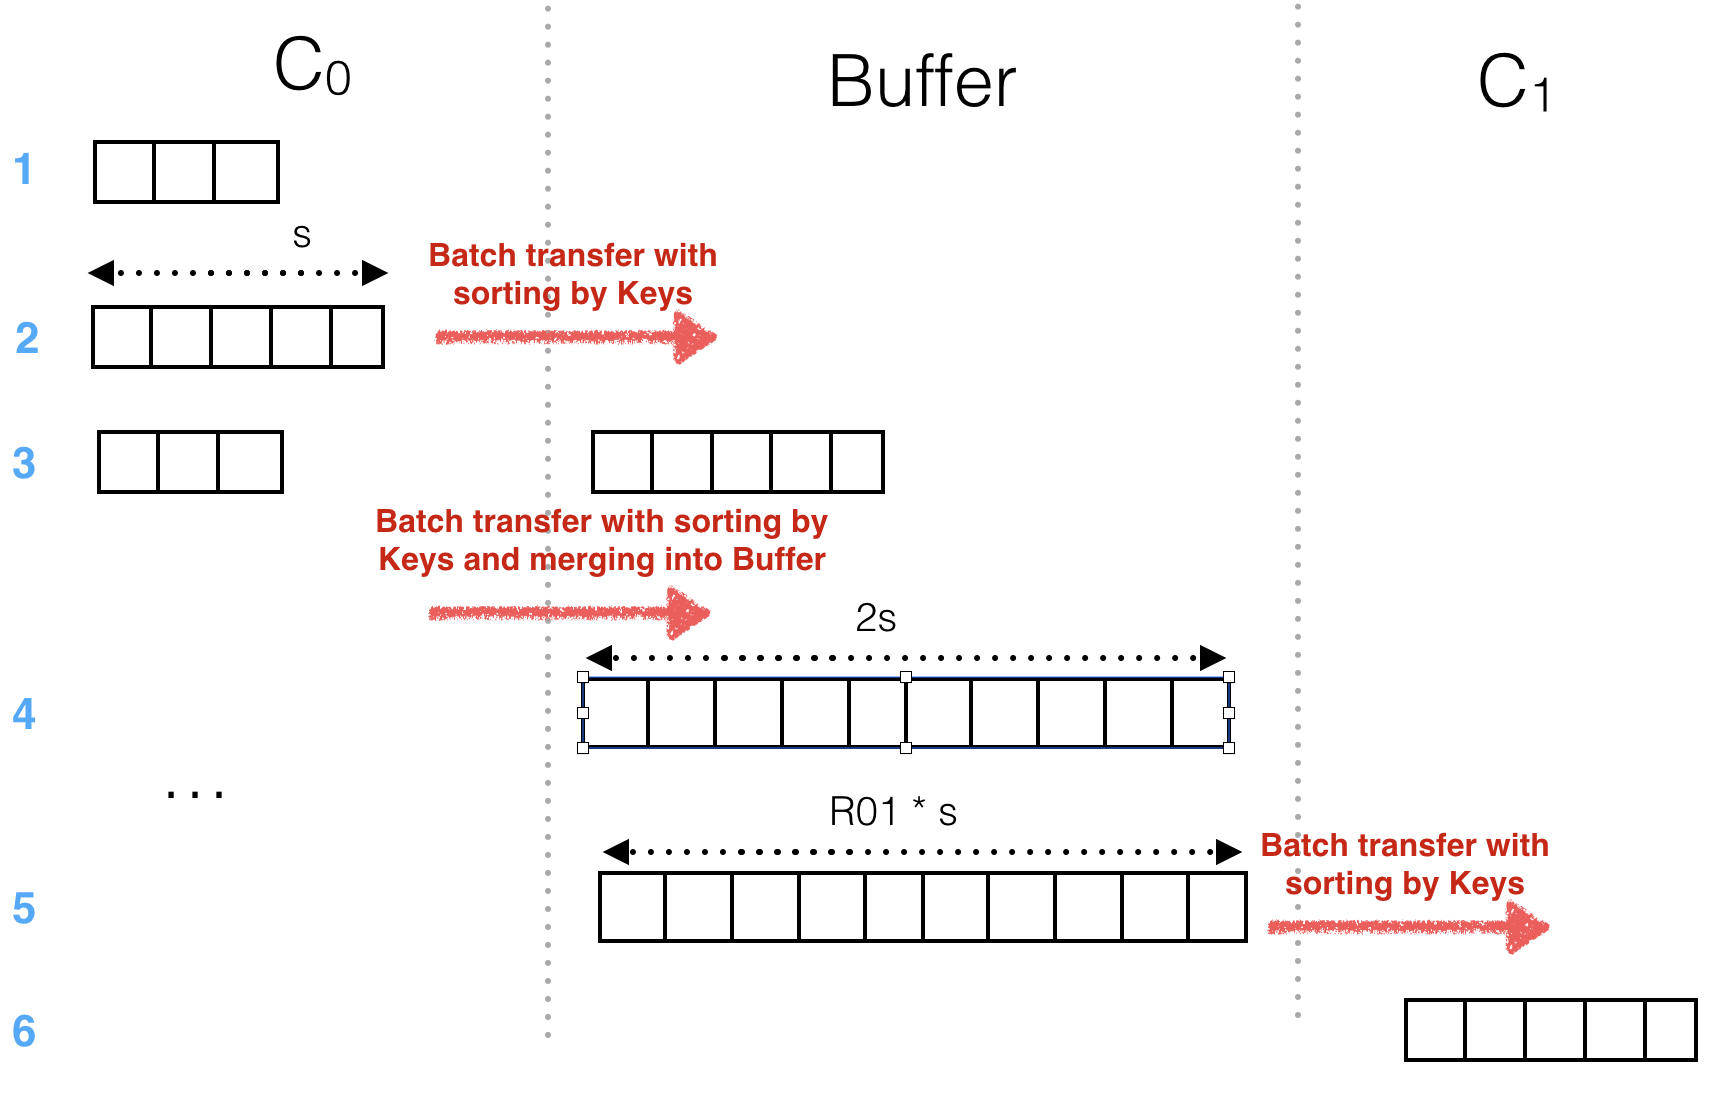
\includegraphics[width=\columnwidth]{img/merge}%
    \caption{Merging Strategy}
    \label{fig:merge}
\end{center}
\end{figure}%

The behavior when flushing one component to the next one is the same for all the component, except for $C_0$ where we also sort it when flushing into the buffer (the deeper components will be sorted already). If the next component is empty, we just fill it, otherwise we merge the incoming array with the existing one to keep it sorted. If the resulting array reaches the deeper component threshold, we flush it to the next component and act recursively. This approach enables to implement right away a multi-components architecture for the LSM tree.

\paragraph{READ}

When reading, we need to search in each component. First, we do a linear scan in $C_0$ and then we look into each deeper component with a binary search.

\subsection{Persistency}

This part presents briefly the storage of the different objects. Each deep component $C_i$ for $i \neq 0$ is stored on disk in 2 files, one for the keys, one for the values. The names of these two files are linked to the name of the LSM tree so we only stored in the metadata the size and the number of elements of each component. The component $C_0$ and the buffer are kept on memory and saved on disk at user demand, as well the metadata of the LSM tree.


\subsection{Implementation details}
\paragraph{Memory Mapped File}

The LSM-trees require an efficient strategy to load the disk components on memory to provide efficient reads and merging operations when appending to the data structure. When reaching the deep components, a lazzy loading is preferred as the number of elements stored in the file becomes bigger (from 100K to 1M). One strategy could be to proceed at the page level of the file and load the required one when searching or merging. Another strategy is to map the file to a region in memory. When applying the \textit{mmap} method, the file can be accessed just like an array in the programm.

\paragraph{Bounds Check}

The LSM-trees are by construction optimized for efficient writes operations. However, reading a key is more expensive as each component need to be scanned. We could make the reads more efficient with some statistics of each component to skip some useless searches. This strategy is particularly efficient when keys in the same range are inserted together in the data structure. Then, each component encompasses a given range and accessing its min-max provides a fast check to reject out-of-range keys. This bounds check strategy is applied on the sorted components as accessing the min/max si simply done by accessing the first and last element of the sorted array.

\paragraph{Fault tolerance}

The structure of the LSM-trees provides a tolerance for fault in case of failure as deep components are stored on disk. As a result, the number of loss elements cannot exceed the memory-based component capacity (here the buffer and $C_0$). We can improve this for workloads where loss is not acceptable. This is done by saving to disk $C_0$ and the LSM-tree metadata after each $K$ append operations and the buffer at each flush. The behavior of the tree on writes becomes then much slower as disk is accessed more often.

\subsection{Bloom Filter}

Another improvement for the read is considered with the use of Bloom filters. These are space-efficient probabilistic data structure use to check if an element is a member of a set. The efficiency of this structure has the drawback of possible false positive checks. The filter uses a pre-defined number of hashes $n_h$ to process a key and set bits with the corresponding hashed indices in a table. The key is present if all the indices are set to 1 but this could happen if the hashed indices of a key have already been set from previous insertions hence the non-null false positive rate.

This structure is used to make the reads faster for elements not present and also as a sanity check for the update and deletes operations. It's currently an external boolean parameter the user need to set.

\subsection{Parallel Reads}

The LSM-trees could be optimized with a concurrent design. The reads operations can naturally be split among different threads, each one searching in parallel on a different component. One key point relies here on the threads synchronization as the concurrent approach becomes efficient when we manage to do less work than with the serial approach to counterbalance the parallel overheads added. As a result, simply waiting for all threads to finish and return the key found in the lowest component will not be efficient. We consider two approaches to tackle this challenge.

The first idea is to kill threads operating on deeper component once the key is found in its lowest component. This is done by joining sequentially the threads starting from the first component on disk. As soon as the key is found, it is the most recent one. We can just kill the working threads as they are on deeper component. This can be done with a handler.

Another approach is to make the thread communicate with each other through a shared variable storing the lowest component on which the key has been found so far. Then each thread checks regularly this variable (for example every $K_p$ iterations of the binary search algorithm) and exit if the value is smaller than its component id. The variable is updated by a component which finds the key while using a semaphore to prevent from race conditions.

\subsection{Alternative Merging Strategy}

To improve the update rate, another merging design is considered. Each component except $C_0$ (with only one unsorted array) contains here a user defined number of sorted arrays $k$. For a given component, the number of elements in each of its $k$ array is given by the total number of elements that can be stored in the component above. If we set as $n$ the size of $C_0$ then the buffer can contain $nk$ elements in total, present in $k$ arrays of $n$ elements; $C_1$ can contain $nk^2$ elements in total, present in $k$ arrays of $nk$ elements and so on.

Here we need to merge the $k$ sorted arrays all at once when flushing a component into the next one. We use the heap sort algorithm where the heap always contain $k$ elements corresponding to the smallest of each sorted array not already flushed. We iterate to extract the minimum and then fill the heap with the next element of the corresponding array.

This variante is more optimized for the updates as less merges are required. However, the data are split among more sorted arrays and the read will be more expansive.

\begin{figure}[H]
\begin{center}
    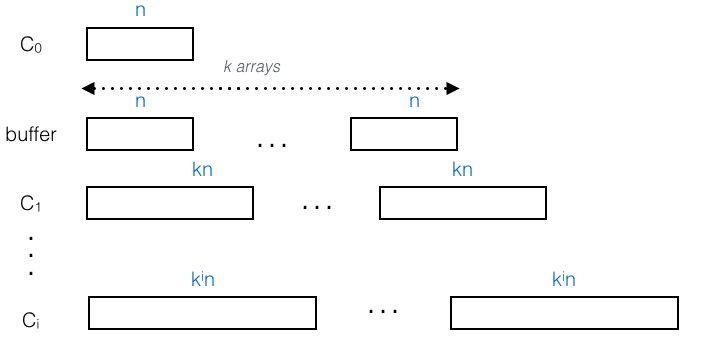
\includegraphics[width=0.4\textwidth]{img/varlsm}
    \caption{Alternative Merging Strategy}
\end{center}
\end{figure}

\section{Experiments}
\subsection{Experiment set up}

For the experiments, we used integers as keys and sequence of characters of size 32 bytes as values. The experiments were executed on a Macbook Pro 2,7 GHz Intel Core i5 with RAM 8 Go 1867 MHz DDR3. We limited the maximum size of a process's data segment at 16 kb to force the system to read from disk when needed. The plots are showed in log scale because of the range of keys tested, but the dependencies are linear.


\subsection{Architecture Benchmarks}

These first experiments aim to show the basic behaviors of an LSM tree with regards to its structure, here defined by the size of its components. Thise size depends on two parameters in our architecture: size of $C_0$ and a ratio $r$ if we assume that $size(\text{buffer}) = r \times size( C_0)$ and for $i>= 1$, $size(C_i) = r^{i+1} \times size(C_0)$.

We display the throughputs for three worlkoads in the plots in figure \ref{fig:archi}, using the 6 different architectures explained in figure \ref{fig:details}: generation of an LSM tree with $10^6$ keys inserted in unsorted order, reads (uniform, skewed on 20\% of the first keys, skewed on 20\% of the last keys) and updates with the same three workloads as the reads. Both the reads and updates occur on an LSM tree intially populated with $10^6$ keys inserted in unsorted order.

\begin{figure}
\centering
\begin{tabular}{|l|l|l|}
\hline
Name   & C0 size & ratio \\ \hline
LSMT 1 & 500     & 3     \\ \hline
LSMT 2 & 500     & 5     \\ \hline
LSMT 3 & 500     & 7     \\ \hline
LSMT 4 & 1000    & 3     \\ \hline
LSMT 5 & 1000    & 5     \\ \hline
LSMT 6 & 1000    & 7     \\ \hline
\end{tabular}
\caption{Architecture details}
\label{fig:details}
\end{figure}

As expected, a larger size of $C_0$ leads to less merges so a better insertion throughput. The best tradeoff for reads \& writes seems to be reached with the configuration 5 for with 22 500 reads/sec and 250 000 updates/sec.

\begin{figure*}

  \begin{minipage}[b]{0.32\textwidth}
    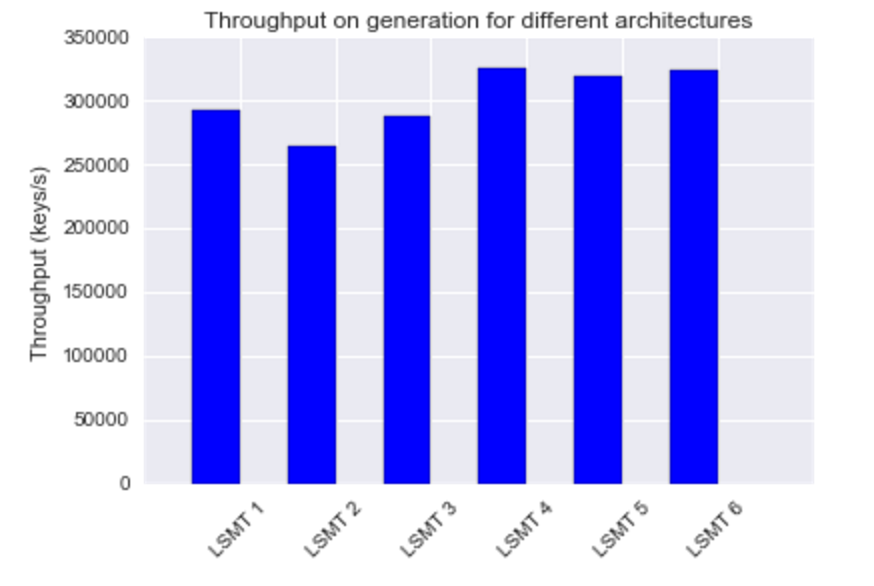
\includegraphics[width=\textwidth]{img/archi_generation}
  \end{minipage}
  \hfill
  \begin{minipage}[b]{0.32\textwidth}
    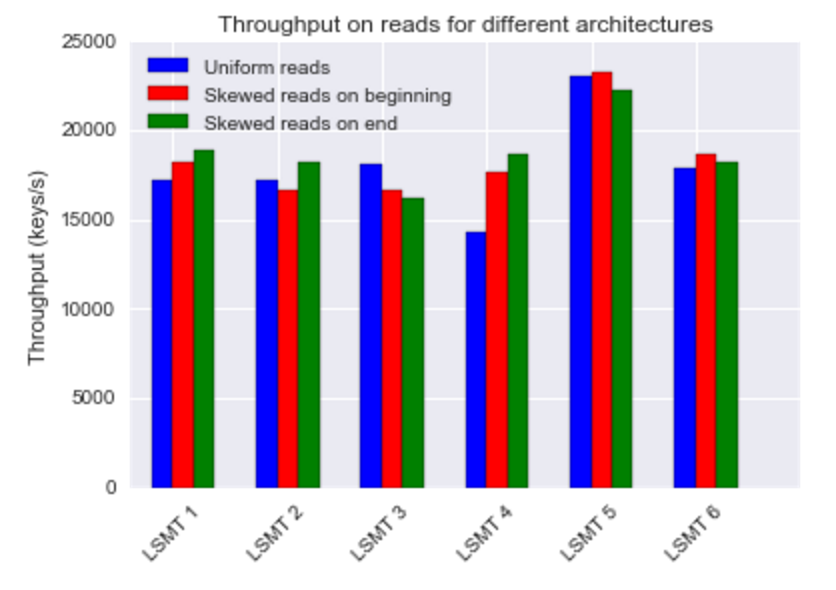
\includegraphics[width=\textwidth]{img/archi_reads}
  \end{minipage}
  \hfill
  \begin{minipage}[b]{0.32\textwidth}
    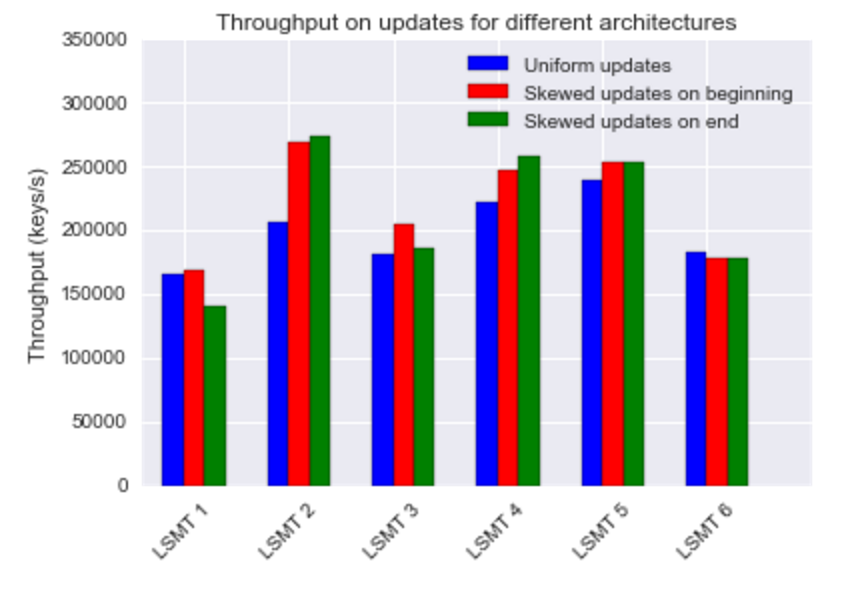
\includegraphics[width=\textwidth]{img/archi_udpates}
  \end{minipage}
  \caption{LSM Tree Behavior on Reads \& Writes with different architectures}
  \label{fig:archi}
\end{figure*}

\subsection{Bloom Filter}
Using a bloom filter presents also a read \& write tradeoff as we have another data sctructure to update at each write but the reads will be much faster if the key is not present.

The behavior of the bloom filter depends also on its parameters: $K$ the number of hashes used and $m$ the number of bits it contains. Given $n$ the number of element to be inserted in the Bloom Filter, the number of hashes that minimizes the false positive probability is $k = \frac{m}{n} \log(2)$.

We ran several workloads of reads and writes to observe the impact of these parameters. The three workloads presented in figure \ref{fig:bloom} are the following: generation of an LSM tree with different number of keys in unsorted order, reads and then updates in an LSM tree intially populated with $10^6$ keys inserted in unsorted order. We tested with different parameters for the Bloom Filter (varying $k$ and $m$) to observe the reads \& writes tradeoffs. We notice that the Bloom filter parameters impact the generation of the LSM Tree. With a large number of hashes each insertion in the bloom filter needs more time. Similarly, with a larger number of bits, more bits will be set to 1 for the same number of keys inserted. We see the same order of performance in the updates plots. The larger configuration (in number of hashes and number of bits) provides slower insertions. For the reads, we tested two workloads per configuration. The full one reads keys which are all present in the tree and the half one contains 50\% of the keys reads outside the tree. This latter workload shows how helpful could be the bloom filter feature, especially with suited parameters. On a large number of keys reads ($10^7$) the time to read dropped by 50\% on the half workload, because each key outside of the tree requires only one comparaison in the read to check if the bit in the bloom filter is set. And the more hashes/number of bits, the less false positive. Without the bloom filter or in case of false positive the entire tree needs to be scanned.

\subsection{Bounds Check}

This final experiment aims to quantify the impact of the bounds check feature added. This feature adds a range check when reading a sorted component. 

We computed the reads throughput for different workloads on an LSM tree populated with 1M keys both in sorted or unsorted order and with or without the bounds check feature. In the results from the figure \ref{ref:bounds}, we first observe the large throughput obtained on an LSM tree populated with sorted keys on a workload skewed on the 20\% last keys. These keys were the last inserted so they are on the "surface" of the tree, mostly in memory so their access is really fast. Another observation is on the impact of the bounds check: it increases the throughput of 20\% on sorted insertions(because the component contain different ranges so the bounds check is always useful) but decreases it from 15\% on unsorted insertions. In this last case, the feature only adds an overhead with the new comparaison when accessing each component as it's less likely that a component contains a specific range. As a result, this feature should be activated when the LSM tree is populated with keys roughly sorted.

\begin{figure}[H]
   \begin{minipage}[b]{\columnwidth}
    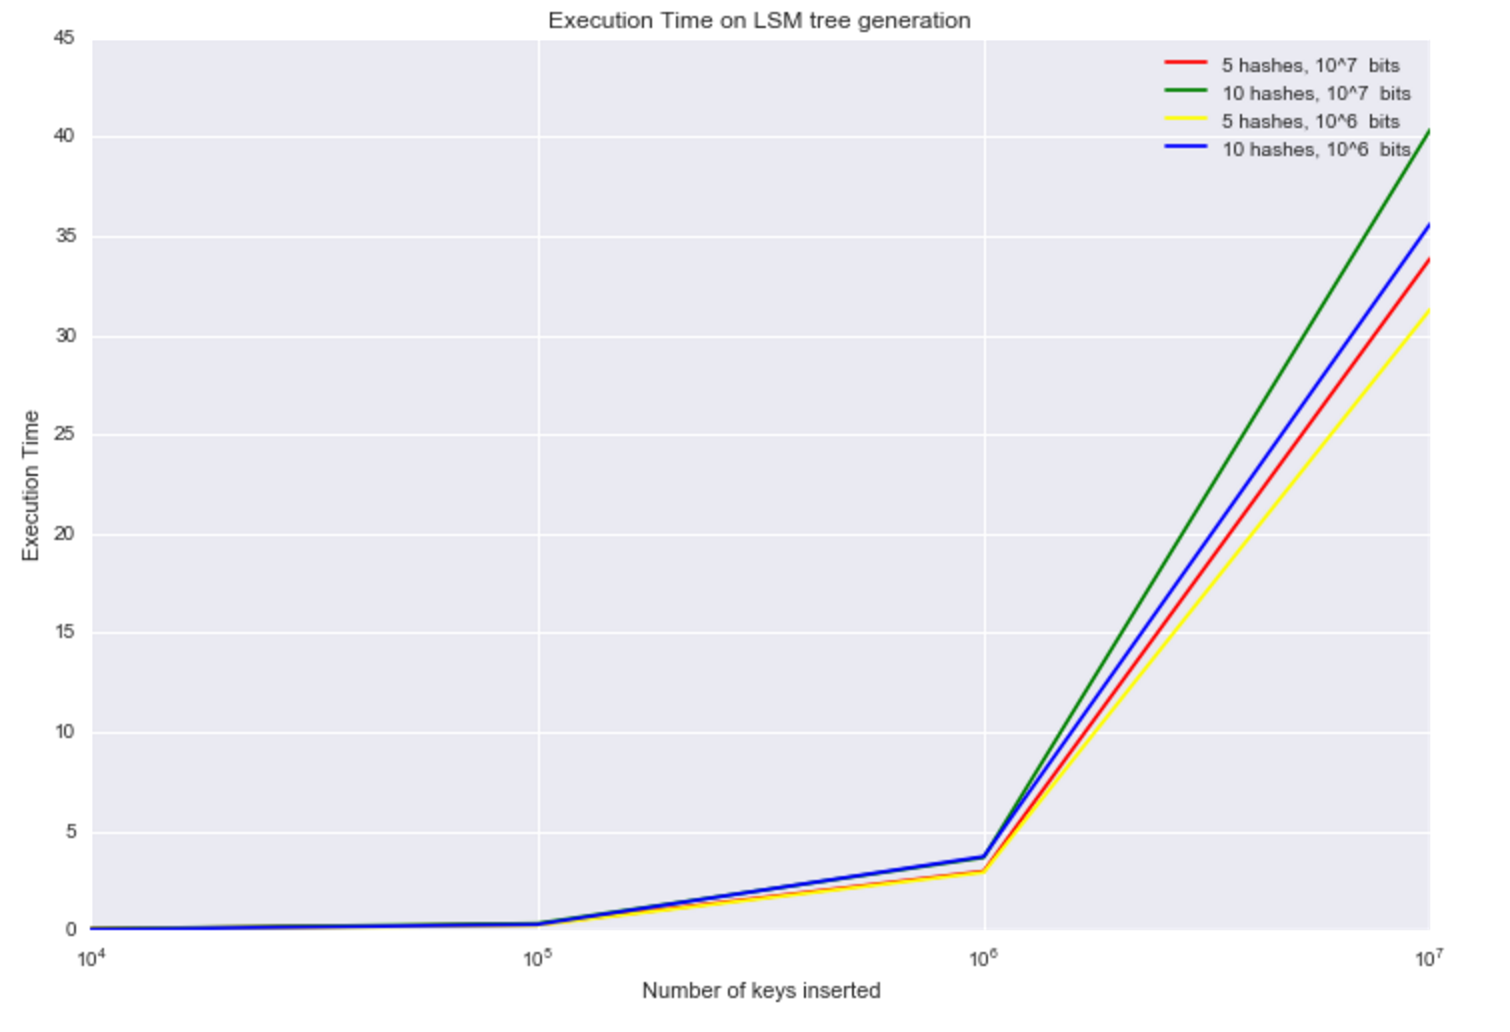
\includegraphics[width=\columnwidth]{img/bloom_gene}
  \end{minipage}
  \begin{minipage}[b]{\columnwidth}
    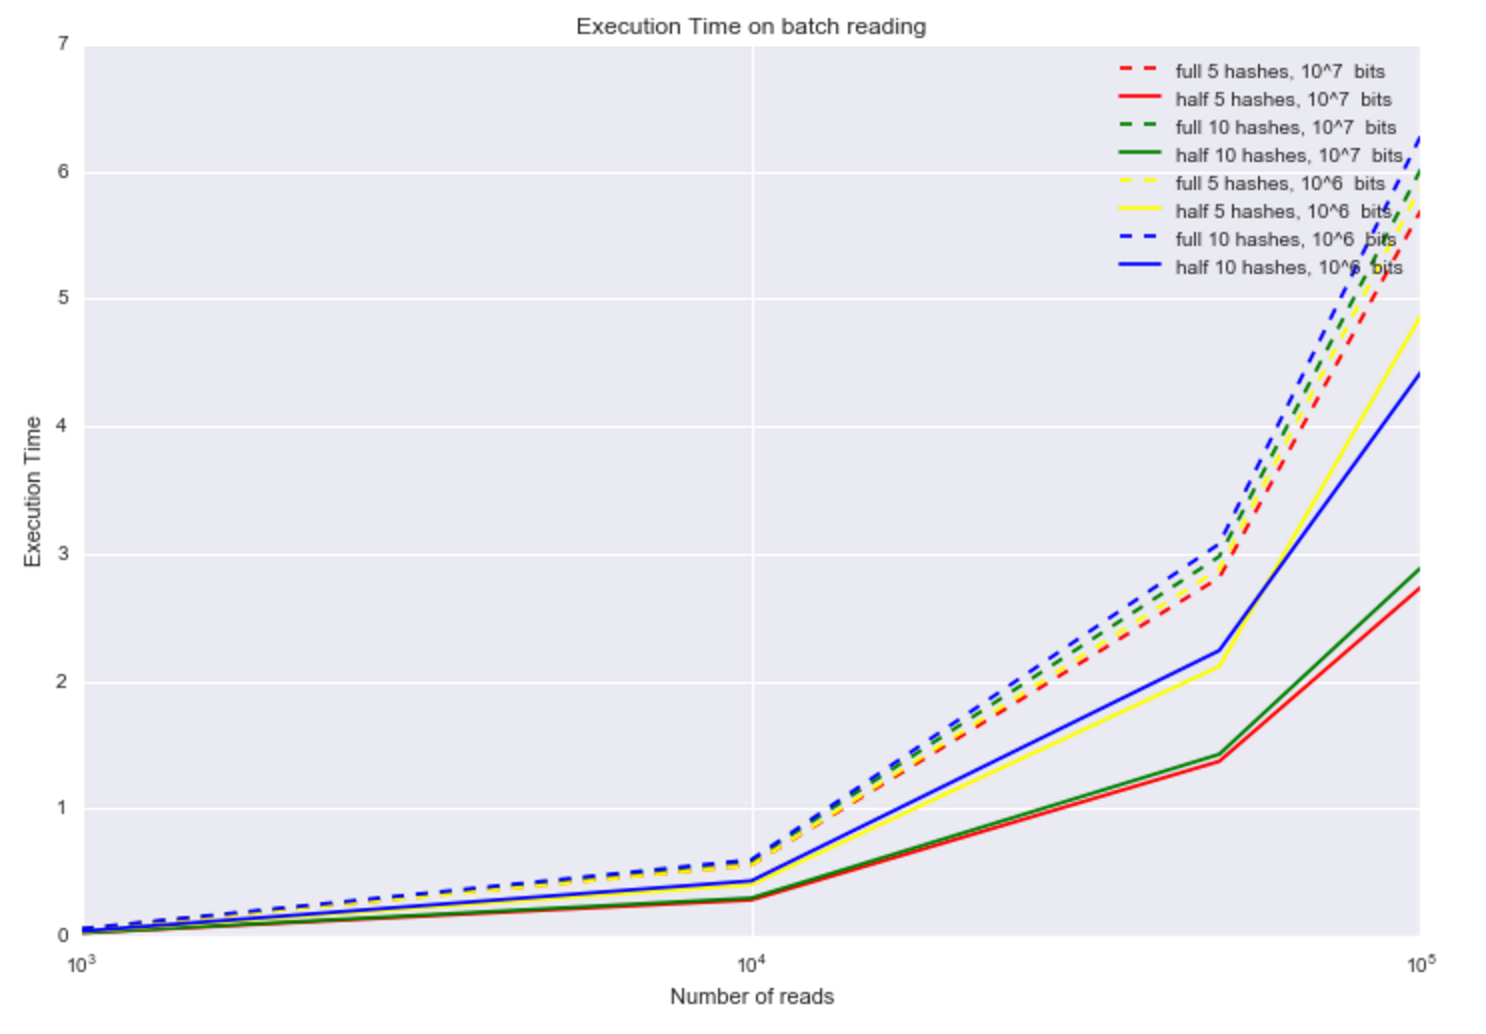
\includegraphics[width=\columnwidth]{img/bloom_reading}
  \end{minipage}
  \begin{minipage}[b]{\columnwidth}
    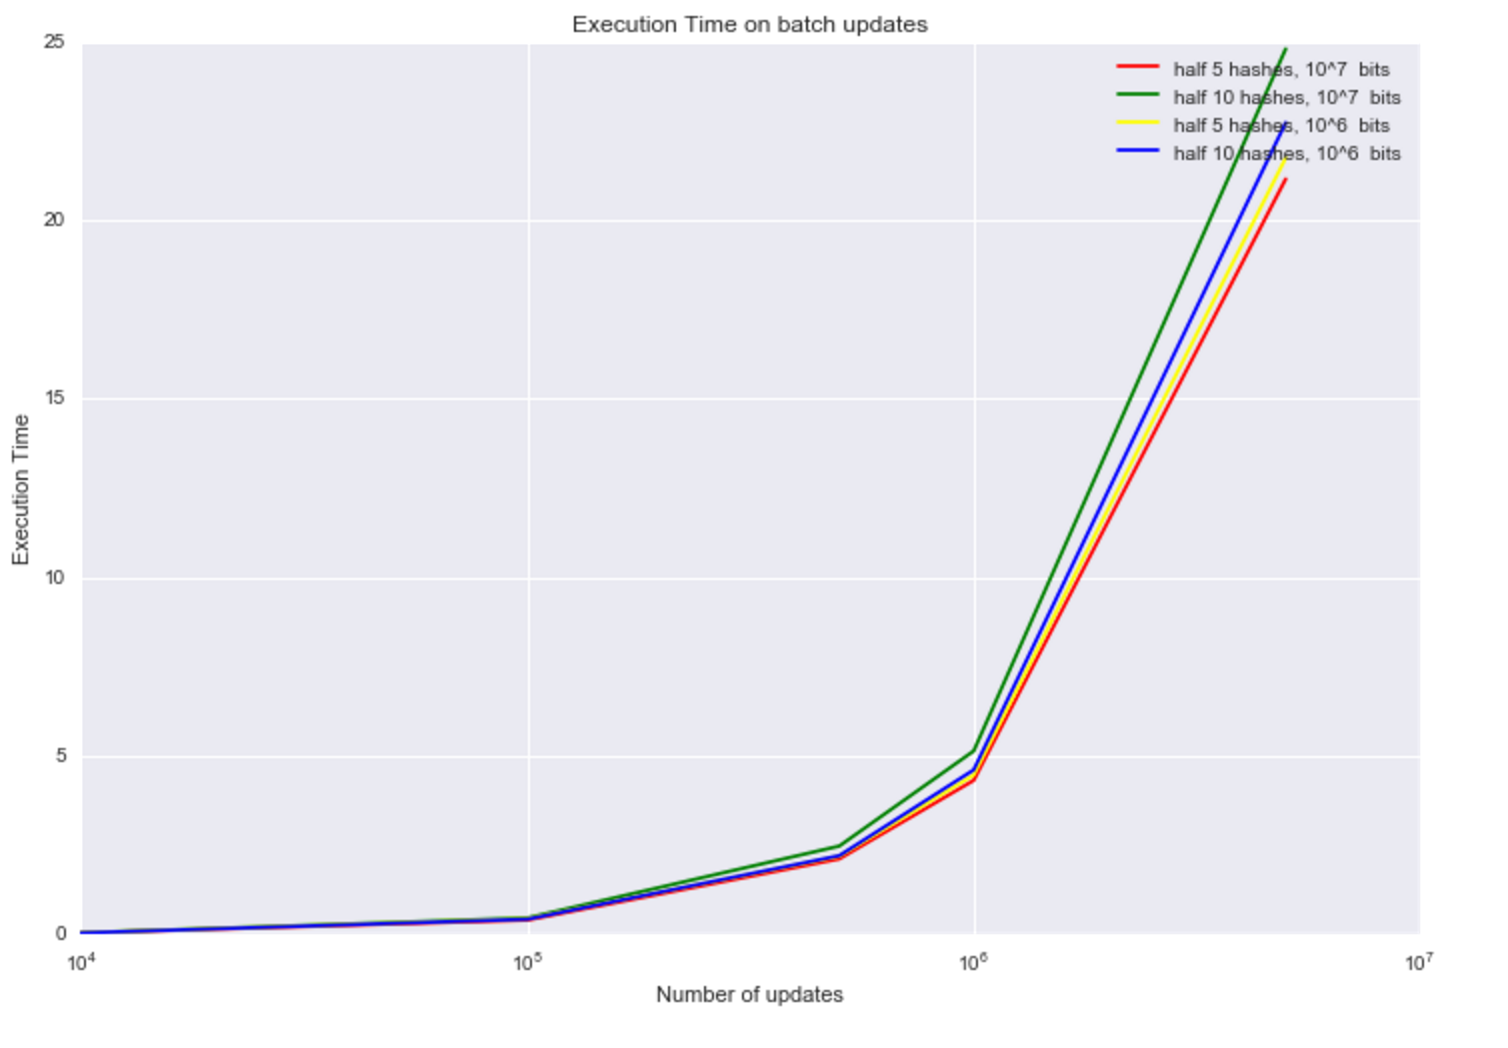
\includegraphics[width=\columnwidth]{img/bloom_updates}
  \end{minipage}
  \caption{LSM Tree Behavior on Reads \& Writes with Bloom filter}
  \label{fig:bloom}
\end{figure}

\begin{figure}
\centering
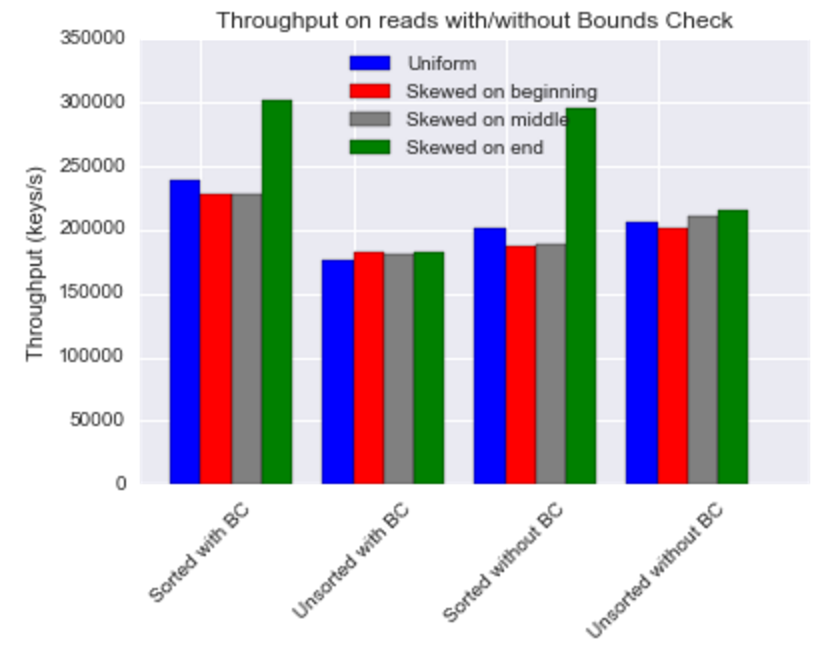
\includegraphics[width=\columnwidth]{img/bounds_reads}
\caption{Bounds Check experiments}
\label{ref:bounds}
\end{figure}



\section{Conclusion}

In conclusion, we implemented a fully functional LSM tree with a merging strategy more optimized for reads as each component contains only one sorted array. We added a Bloom Filter and bounds check to make the reads even more efficient. Future work could be to finish the implementation of the alternative merging strategy to add a parameter in the LSM tree defining which strategy to use. Another step is to validate the parallel implementation with more experiments. The current implementation, tested on a 4 core Macbook Pro, did not provide better performance than the serial implementaiton. Another experiment to validate the alternative merging strategy, theoretically more optimized for writes, could be considered too.

\bibstyle{abbrv}
\bibliography{sigproc}

\end{document}
